% !TEX TS-program = pdflatexmk
% !TEX encoding = UTF-8 Unicode
\documentclass{beamer}
\usepackage[utf8]{inputenc}
\usepackage{helvet}
\usepackage[english, ngerman]{babel}
\usepackage{nameref}
\usepackage{listings}
\usepackage{amsmath}
\usepackage{amssymb}
\usepackage{graphicx}

\usepackage{pgf}
\usepackage{tikz}

\usepackage{../styles/pgf-umlcd}
\usepackage{pgfplots, pgfplotstable}
%\pgfplotsset{compat=1.8}
%\usepgfplotslibrary{statistics}

\usecolortheme{tum}
\useoutertheme{tum}

\setbeamerfont{author}{size=\footnotesize}
\setbeamerfont{date}{size=\scriptsize}
\setbeamerfont{date}{size=\scriptsize}

\useinnertheme{rectangles}

\usepackage{pgf}  
\usepackage{tikz}
\logo{\pgfputat{\pgfxy(-0.2, 8.9)}{\pgfbox[right,top]{
\begin{tikzpicture}[y=0.38pt, x=0.38pt,yscale=-1, inner sep=0pt, outer sep=0pt]
\begin{scope}[cm={{1.25,0.0,0.0,-1.25,(0.0,35.4325)}}]
    \path[fill=tum,nonzero rule] (4.8090,23.2950) -- (4.8090,-0.0020) --
      (9.8590,-0.0020) -- (9.8590,23.2600) -- (15.4730,23.2600) -- (15.4730,-0.0020)
      -- (31.5390,-0.0020) -- (31.5390,23.0140) -- (37.2580,23.0140) --
      (37.2580,0.0060) -- (42.5550,0.0060) -- (42.5550,23.0140) -- (48.3440,23.0140)
      -- (48.3440,0.0060) -- (53.6410,0.0060) -- (53.6410,28.3460) --
      (26.4530,28.3460) -- (26.4530,5.1580) -- (20.6290,5.1580) -- (20.6290,28.3110)
      -- (-0.0000,28.3110) -- (-0.0000,23.2950) -- (4.8090,23.2950) -- cycle;
\end{scope}
\end{tikzpicture}
}}}

\AtBeginSection[]
{
	\begin{frame}
		\frametitle{Agenda}
		\tableofcontents[currentsection]
	\end{frame}
}

\setbeamertemplate{title page}
{
	\vbox{}
	\vfill
	\begin{flushleft}
		\begin{beamercolorbox}[sep=8pt,left]{title}
			\usebeamerfont{title}\inserttitle\par%
			\ifx\insertsubtitle\@empty%
			\else%
				\vskip0.25em%
				{\usebeamerfont{subtitle}\usebeamercolor[fg]{subtitle}\insertsubtitle\par}%
			\fi%
    	\end{beamercolorbox}%
    	\vskip1em\par
		\begin{beamercolorbox}[sep=8pt,left]{author}
		\usebeamerfont{author}\insertauthor
		\end{beamercolorbox}
		\begin{beamercolorbox}[sep=8pt,left]{institute}
		\usebeamerfont{institute}\insertinstitute
		\end{beamercolorbox}
		\begin{beamercolorbox}[sep=8pt,left]{date}
		\usebeamerfont{date}\insertdate
		\end{beamercolorbox}\vskip0.5em
		{\usebeamercolor[fg]{titlegraphic}\inserttitlegraphic\par}
	\end{flushleft}
	\vfill
}

\mode<presentation>

\title{Evaluierung und Vorhersage von Ausf\"uhrungszeiten f\"ur OpenCL-basierte Berechnungen auf GPGPU-Systemen}
\subtitle{Abschlussvortrag}

\author{Alexander Pöppl}
\institute[]{Lehrstuhl für Sprachen und Beschreibungsstrukturen \\Fakultät für Informatik\\ Technische Universität München}

\begin{document}

\begin{frame}
	\titlepage
\end{frame}

\begin{frame}
	\tableofcontents
\end{frame}

\section{Motivation}
\label{sect:motivation}

\begin{frame}
	\frametitle{\nameref{sect:motivation}}
	\begin{figure}
		\centering
		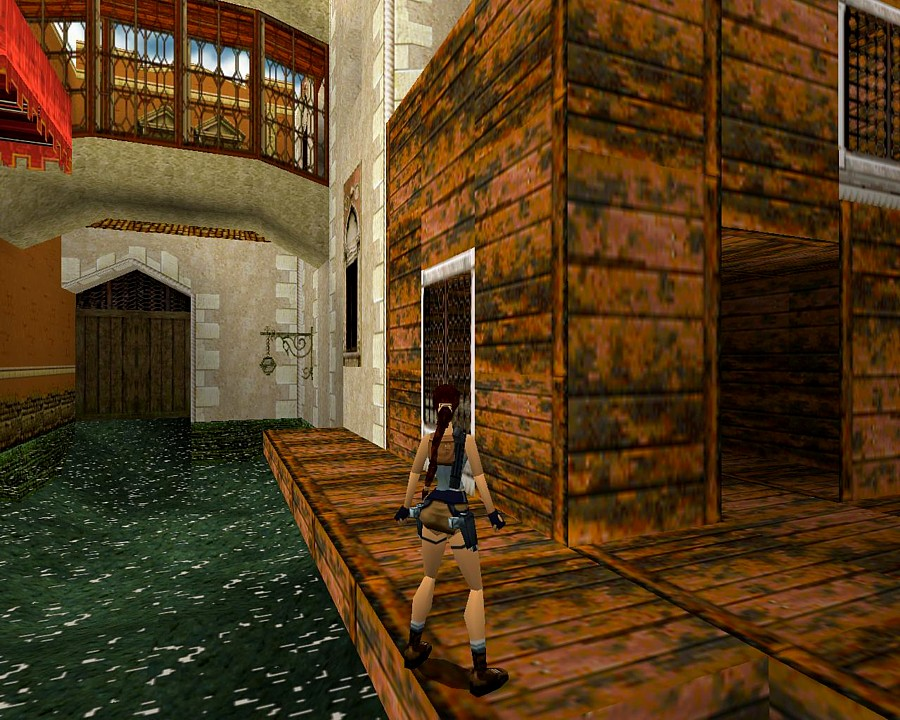
\includegraphics[width=.75\linewidth]{../images/oldGraphics}
	\end{figure}	
\end{frame}

\begin{frame}
	\frametitle{\nameref{sect:motivation}}
	\begin{figure}
		\centering
		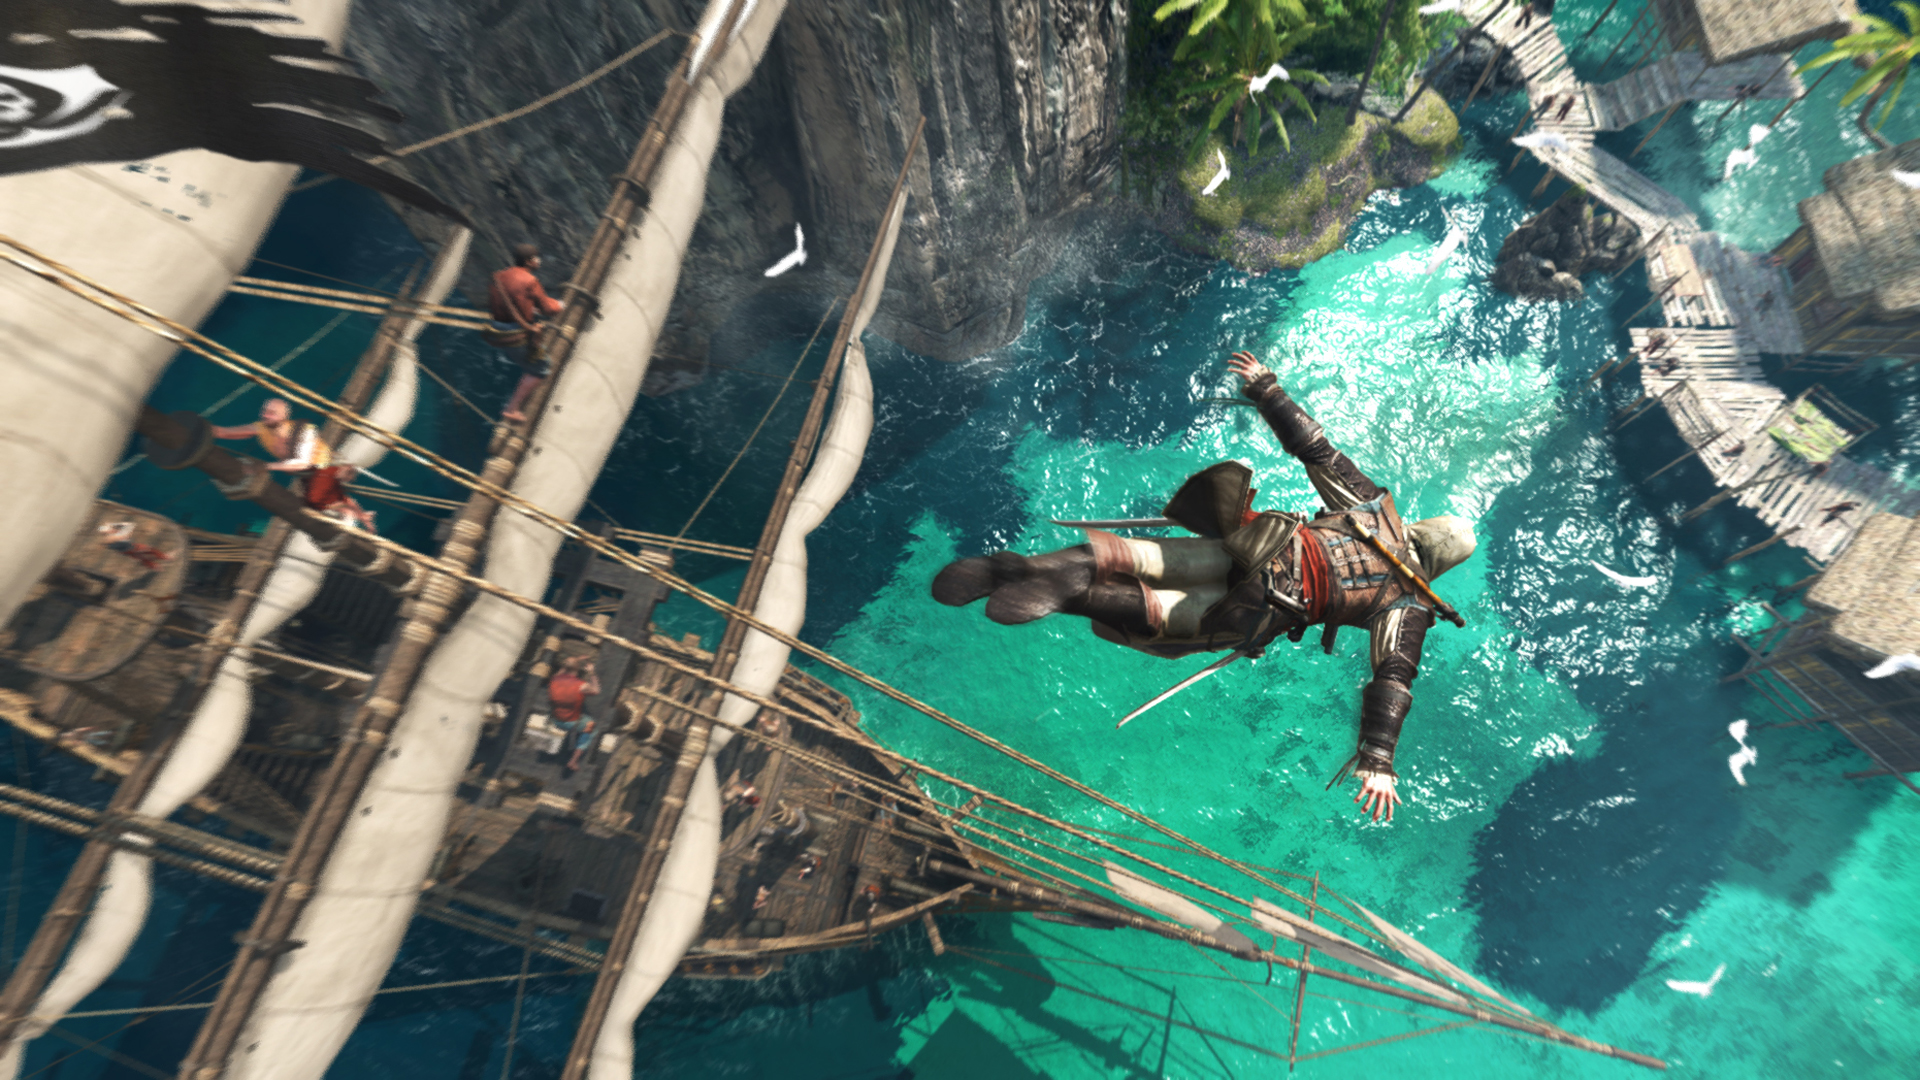
\includegraphics[width=.95\linewidth]{../images/modernGraphics}
	\end{figure}	
\end{frame}

\begin{frame}
	\frametitle{\nameref{sect:motivation}}
	\begin{itemize}
		\item Bemerkenswerte Entwicklungen im Bereich der GPUs
		\item Vorteile von GPUs:
		\begin{itemize}
			\item Hochgradig Parallel
			\item Schnelle Speicherzugriffe
			\item Spezialisiert auf Berechnungen auf großen Datensätzen
		\end{itemize}
		\pause
		\item \emph{General Purpose GPU Programming}
		\item \emph{Signifikante Performancegewinne möglich.}
	\end{itemize}
\end{frame}

\begin{frame}
	\frametitle{\nameref{sect:motivation}}
	\begin{itemize}
		\item Programmierung für die GPU komplexer als für die CPU
		\item Stark an die Hardwarestruktur angelehnt
		\pause
		\item Berechnung auf der GPU nicht zwangsläufig schneller
		\item Overhead für Transfer von Daten zur GPU
		\pause
		\item Compiler soll entscheiden, wo Berechnung ausgeführt wird
		\item Entscheidung basierend auf erwarteten Ausführungszeiten der Berechnungen auf GPU und CPU
		\pause
		\item \emph{Modellierung der Ausführungszeiten auf der GPU}
	\end{itemize}
\end{frame}

\begin{frame}
	\frametitle{\nameref{sect:motivation}}
	\begin{figure}[h]
		\begin{center}
			\begin{tikzpicture}
				\begin{loglogaxis}[ 	xlabel=Anzahl Elemente im Array, 
								ylabel=Zeit in $\mu s$,
								legend entries={\tiny CPU Gesamt, \tiny GPU Gesamt, \tiny GPU Ausführung},
								legend style={at={(1.03, 0.5)}, anchor=west}]
					\addplot [red, error bars/.cd, y dir=both, y explicit] table [x=elements, y=cpu, y error=cpuStdDev]{../data/cpugpu.csv};
					\addplot [blue, error bars/.cd, y dir=both, y explicit] table [x=elements, y=gpu, y error=gpuStdDev]{../data/cpugpu.csv};
					\addplot [green, error bars/.cd, y dir=both, y explicit] table [x=elements, y=run, y error=runStdDev]{../data/cpugpu.csv};
				\end{loglogaxis}
			\end{tikzpicture}
		\end{center}
	\end{figure}
\end{frame}

\section{Theorie}
\label{sect:theory}

\begin{frame}
	\frametitle{\nameref{sect:theory}}
	\framesubtitle{OpenCL}
	\begin{itemize}
		\item Offener Standard zur Durchführung von parallelen Berechnungen auf heterogenen Systemen
		\item Unterstützt GPUs, CPUs, Accelerators
		\item Implementierungen u.a. von Intel, AMD, NVidia, Apple
		\item Unterstützt Taskparallelität, Datenparallelität
	\end{itemize}
\end{frame}

\begin{frame}
	\frametitle{\nameref{sect:theory}}
	\framesubtitle{OpenCL}
	\begin{itemize}
		\item \textbf{Platform:} ``Konventionelle'' Ausführungsumgebung. Kann Devices nutzen, um Berechnungen durchzuführen.
		\item \textbf{Device:} Gerät, auf dem OpenCL-Code ausgeführt wird
		\item \textbf{Kernel:} Die Funktion, die auf der GPU ausgeführt wird. Muss kompiliert werden.
		\item \textbf{Memory:} Die Daten, die der Kernel nutzt. Müssen transferiert werden.
	\end{itemize}
\end{frame}

\begin{frame}
	\frametitle{\nameref{sect:theory}}
	\framesubtitle{OpenCL-Plattformmodell}
	\begin{figure}
		\begin{center}
			\resizebox{.75\textwidth}{.75\textheight}{
				\begin{tikzpicture}
					\begin{object}{macbook - Platform}{10.5 ,-4.75}
						\attribute{name = ``Apple''}
						\attribute{vendor = ``Apple''} 
					\end{object}
					\begin{object}{gt650 - Device}{5 ,0}
						\attribute{name = ``GeForce GT650M''}
						\attribute{vendor = ``NVIDIA''} 
						\attribute{type = GPU}
					\end{object}
					\begin{object}{hd4000 - Device}{5 ,-4.5}
						\attribute{name = ``HD Graphics 4000''}
						\attribute{vendor = ``Intel''} 
						\attribute{type = GPU}
					\end{object}
					\begin{object}{corei7 - Device}{5 ,-9}
						\attribute{name = ``Intel(R) Core(TM) i7-3740QM CPU @ 2.70GHz''}
						\attribute{vendor = ``Intel''} 
						\attribute{type = CPU}
					\end{object}
					\begin{object}[text width=3.5cm]{n0 - ExecutionUnit}{0 ,0}
						\attribute{processingElements = 256}
					\end{object}
					\begin{object}[text width=3.5cm]{n1 - ExecutionUnit}{0 ,2}
						\attribute{processingElements = 256}
					\end{object}
					\begin{object}[text width=3.5cm]{h0 - ExecutionUnit}{0 ,-3.25}
						\attribute{processingElements = 16}
					\end{object}
					\node[draw] at (0,-5.5) {...};
					\begin{object}[text width=3.75cm]{h15 - ExecutionUnit}{0 ,-6}
						\attribute{processingElements = 16}
					\end{object}
					\begin{object}[text width=3.5cm]{i0 - ExecutionUnit}{0 ,-8.5}
						\attribute{processingElements = 4}
					\end{object}
					\node[draw] at (0,-10.5) {...};
					\begin{object}[text width=3.5cm]{i7 - ExecutionUnit}{0 ,-11}	
						\attribute{processingElements = 4}
					\end{object}
					\association{macbook - Platform}{}{}{gt650 - Device}{}{}		
					\association{macbook - Platform}{}{}{hd4000 - Device}{}{}		
					\association{macbook - Platform}{}{}{corei7 - Device}{}{}
					\association{gt650 - Device}{}{}{n0 - ExecutionUnit}{}{}
					\association{gt650 - Device}{}{}{n1 - ExecutionUnit}{}{}
					\association{hd4000 - Device}{}{}{h0 - ExecutionUnit}{}{}
					\association{hd4000 - Device}{}{}{h15 - ExecutionUnit}{}{}
					\association{corei7 - Device}{}{}{i0 - ExecutionUnit}{}{}
					\association{corei7 - Device}{}{}{i7 - ExecutionUnit}{}{}
				\end{tikzpicture}
			}
			\label{fig:platform_example}
		\end{center}	
	\end{figure}
\end{frame}

\begin{frame}
	\frametitle{\nameref{sect:theory}}
	\framesubtitle{OpenCL-Ausführungsmodell}
	\begin{block}{Begriffe}
		\begin{itemize}
			\item \textbf{Work-Item:} Einzelner Thread, ein Durchlauf des Kernels
			\item \textbf{Work-Group:} Gruppe von Work-Items, die nebenläufig ausgeführt wird
		\end{itemize}
	\end{block}
	\begin{block}{Einschränkungen}
		\begin{itemize}
			\item Es werden immer nur Work-Items einer Work-Group gleichzeitig ausgeführt
			\item Vor Beginn der Ausführung einer neuen Work-Group muss die vorhergehende abgeschlossen sein
			\item $n_{Work-Items} \operatorname{mod} s_{Work-Group} = 0$
		\end{itemize}
	\end{block}
\end{frame}

\begin{frame}
	\frametitle{\nameref{sect:theory}}
	\framesubtitle{OpenCL-Speichermodell}
	\begin{figure}
		\begin{center}
			\includegraphics[width=0.75\linewidth]{../images/memory_hierarchy}
		\end{center}
		\label{fig:theory_memory_hierarchy}
	\end{figure}
\end{frame}

\begin{frame}
	\frametitle{\nameref{sect:theory}}
	\framesubtitle{funkyIMP}
	\begin{block}{}
		\begin{itemize}
			\item Sprachfeature von Interesse: \emph{Domain Iterations}
			\pause
			\item Iteration über Mehrdimensionale Arrays
		\end{itemize}
	\end{block}
	\begin{exampleblock}{}
		\lstinputlisting[language=java, morekeywords={domain}, basicstyle=\small]{../code/funkyArray2.funky}
	\end{exampleblock}
\end{frame}

\section{Erweiterung des funkyIMP Compilers}
\label{sect:extensions}

\begin{frame}
	\frametitle{\nameref{sect:extensions}}
	\begin{itemize}
		\item Generierung des Codes aufseiten des Hosts
			\begin{itemize}
				\item Sammeln der Variablen
				\item Code zum Kompilieren des Kernels
				\item Transfer der Daten zur GPU
				\item Ausführung des Kernels
				\item Rücktransfer des Ergebnisses
			\end{itemize}
			\pause
		\item Übersetzung der Domain Iteration in einen OpenCL-Kernel
			\begin{itemize}
				\item Kernel Header
				\item Expression innerhalb der Domain Iteration
			\end{itemize}
	\end{itemize}
\end{frame}

\begin{frame}
	\frametitle{\nameref{sect:extensions}}
	\framesubtitle{Beispiel}
	\lstinputlisting[language=java, morekeywords={domain}, basicstyle=\small]{compExp.funky}
\end{frame}

\begin{frame}
	\frametitle{\nameref{sect:extensions}}
	\framesubtitle{Beispiel - Code auf Hostseite}
	\lstinputlisting[language=c++, firstline=12, lastline=22, basicstyle=\small]{../code/exampleDomain.cpp}
\end{frame}

\begin{frame}
	\frametitle{\nameref{sect:extensions}}
	\framesubtitle{Beispiel - Code auf Hostseite (Fortsetzung)}
	\lstinputlisting[language=c++, firstline=24, lastline=40, basicstyle=\small]{../code/exampleDomain.cpp}
\end{frame}

\begin{frame}
	\frametitle{\nameref{sect:extensions}}
	\framesubtitle{Beispiel - Code auf Hostseite (Fortsetzung)}
	\lstinputlisting[language=c++, firstline=42, lastline=49, basicstyle=\small]{../code/exampleDomain.cpp}
\end{frame}

\begin{frame}
	\frametitle{\nameref{sect:extensions}}
	\framesubtitle{Beispiel - Code auf Hostseite (Fortsetzung)}
	\lstinputlisting[language=c++, firstline=51, lastline=65, basicstyle=\small]{../code/exampleDomain.cpp}
\end{frame}

\begin{frame}
	\frametitle{\nameref{sect:extensions}}
	\framesubtitle{Beispiel - Kernel Code}
	\lstinputlisting[language=c, morekeywords={__kernel, __global}, lastline=10, basicstyle=\small]{../code/exampleKernel.cl}
\end{frame}

\begin{frame}
	\frametitle{\nameref{sect:extensions}}
	\framesubtitle{Beispiel - Kernel Code (Fortsetzung)}
	\lstinputlisting[language=c, morekeywords={__kernel, __global}, firstline=11, basicstyle=\small]{../code/exampleKernel.cl}
\end{frame}

\section{Benchmark Suite}
\label{sect:suite}

\begin{frame}
	\frametitle{\nameref{sect:suite}}
	\begin{itemize}
		\item Suite zur Durchführung von Benchmarks zur experimentellen Bestimmung der Ausführungszeiten
		\item Führt $n$ Benchmarks auf einem Device aus, für verschiedene Werte (z.B Größe der Work-Group, Größe des Speichers, Anzahl Operationen)
		\item Mehrmalige Durchführung, solange bis Standardfehler kleiner als angegeben
	\end{itemize}
\end{frame}

\section{Ausführungszeitmodell}
\label{sect:model}

\subsection{Datentransfer}
\label{sect:model_transfer}

\begin{frame}
	\frametitle{\nameref{sect:model}}
	\framesubtitle{\nameref{sect:model_transfer}}
	\begin{itemize}
		\item GPU typischerweise über PCI Express angebunden
		\item Einfluss von Bandbreite von PCI Express BUS
		\item Einfluss von Latenz von PCI Express BUS, Speicheranbindung, Speicher
	\end{itemize}
\end{frame}

\begin{frame}
	\frametitle{\nameref{sect:model}}
	\framesubtitle{\nameref{sect:model_transfer} - Experiment}
	\begin{itemize}
		\item Transfer von sukzessiv größer werdenden Speicherblöcken
		\item Messung der Zeit für Transfer zu und von der GPU
		\item $128kB \rightarrow 16MB$, in Schritten zu $128kB$
	\end{itemize}
\end{frame}

\begin{frame}
	\frametitle{\nameref{sect:model}}
	\framesubtitle{\nameref{sect:model_transfer} - Experiment}
	\begin{figure}
		\begin{center}
			\begin{tikzpicture}
				\begin{axis}[	xlabel=Anzahl DWords, 
							ylabel=Zeit in $\mu s$,
							legend entries={\tiny Zur GPU, \tiny Von der GPU, \tiny Zur GPU interpoliert, \tiny Von der GPU interpoliert},
							legend style={at={(1.03, 0.5)}, anchor=west}]
					\addplot [blue, mark=halfcircle, error bars/.cd, y dir=both, y explicit] table [x=NumElements, y=ToGpu, y error=ToGpuStdDev]{../data/copyGPUData.csv};
					\addplot [green, mark=halfcircle, error bars/.cd, y dir=both, y explicit] table [x=NumElements, y=FromGpu, y error=FromGpuStdDev]{../data/copyGPUData.csv};
					\addplot [red, domain=1e3:67e6, samples=5] {0.00351162*x+516.413};
					\addplot [orange, domain=1e3:67e6, samples=5] {0.000537919*x+173.626};
				\end{axis}
			\end{tikzpicture}
			\label{fig:model_gpu_transfer}
		\end{center}
	\end{figure}
\end{frame}

\begin{frame}
	\frametitle{\nameref{sect:model}}
	\framesubtitle{\nameref{sect:model_transfer}}
	
	\begin{block}{Ergebnis}
		\begin{itemize}
			\item Linear abhängig von der Speichergröße
			\item $T_{trans}(x) = b^{-1} * x + l_{prop}$
		\end{itemize}
	\end{block}
	\begin{block}{MacBook Pro}
		\begin{align*}
			T_{\rightarrow GPU_{rMBP}} &= 0.0035800\mu s * x + 516.41\mu s\\
			T_{\leftarrow GPU_{rMBP}} &= 0.00053337\mu s * x + 173,63\mu s
		\end{align*}
	\end{block}
\end{frame}

\subsection{Leere Kernel}
\label{sect:model_empty}

\begin{frame}
	\frametitle{\nameref{sect:model}}
	\framesubtitle{\nameref{sect:model_empty}}
	\begin{itemize}
		\item Basiskosten für Kernelausführungen
		\item Ausführung von leeren Kernel auf sukzessiv wachsenden Speichersegmenten
		\item Messung der Ausführungszeiten
		\item $128kB \rightarrow 16MB$, in Schritten zu $128kB$
	\end{itemize}
\end{frame}

\begin{frame}
	\frametitle{\nameref{sect:model}}
	\framesubtitle{\nameref{sect:model_empty} - Experiment}
	\begin{figure}
		\begin{center}
			\begin{tikzpicture}
				\begin{axis}[	xlabel=Anzahl Work-Items, 
							ylabel=Zeit in $\mu s$,
							legend entries={\tiny Kernellaufzeit, \tiny Interpolierte Funktion},
							legend style={at={(1.03, 0.5)}, anchor=west}]
					\addplot [blue, error bars/.cd, y dir=both, y explicit] table [x=NumberOfElements, y=Runtime, y error=StandardDeviation]{../data/emptyKernel.csv};
					\addplot [red, domain=1e3:16.7e6, samples=5] {0.000189885660433182 * x + 5.72651881044402};
				\end{axis}
			\end{tikzpicture}
		\end{center}
	\end{figure}
\end{frame}

\begin{frame}
	\frametitle{\nameref{sect:model}}
	\framesubtitle{\nameref{sect:model_empty}}
	\begin{block}{Ergebnis}
		\begin{itemize}
			\item Linear abhängig von der Anzahl Work-Items
			\item $T_{Base}(x) = t_{Element}*x+c$
		\end{itemize}	
	\end{block}
	\begin{block}{MacBook Pro}
		\begin{align*}
			T_{Base_{rMBP}} &= 0.18989ns * x + 5.7265\mu s
		\end{align*}
	\end{block}
\end{frame}


\subsection{Größe der Work-Group}
\label{sect:model_wgsize}

\begin{frame}
	\frametitle{\nameref{sect:model}}
	\framesubtitle{\nameref{sect:model_wgsize}}
	\begin{itemize}
		\item Langsamere Ausführungszeit für manche Kernel beobachtet
		\item Experiment: Ausführung eines Kernels auf einer fixen Anzahl Elemente mit sukzessiv wachsender Größe der Work-Group
		\item Messung der Ausführungszeiten
		\item $1 \rightarrow s_{Work-Group_{max}}$
	\end{itemize}
\end{frame}

\begin{frame}
	\frametitle{\nameref{sect:model}}
	\framesubtitle{\nameref{sect:model_wgsize} - Experiment}
	\begin{figure}[p]
		\begin{center}
			\begin{tikzpicture}
				\begin{axis}[	xlabel=Anzahl Work-Items pro Work-Group, 
							ylabel=Zeit in $\mu s$,
							legend entries={\tiny Kernellaufzeit, \tiny Interpolierte Funktion},
							legend style={at={(1.03, 0.5)}, anchor=west}]
					\addplot [green] table [x=WorkgroupSize, y=Runtime]{../data/wgSize.csv};
					\addplot [red, domain=1:1e3, samples=500] {18192*exp(-x/12.2112414869873)+36412*exp(-x/2.28329383738342)+1395.1};
				\end{axis}
			\end{tikzpicture}
		\end{center}
	\end{figure}
\end{frame}

\begin{frame}
	\frametitle{\nameref{sect:model}}
	\framesubtitle{\nameref{sect:model_wgsize}}
	\begin{block}{Ergebnis}
		\begin{itemize}
			\item Invers exponentiell abhängig von der Größe der Work-Group
			\item $M_{WG}(x) = \underbrace{B_1*e^{\frac{-x}{t_1}}}_\text{A} + \underbrace{B_2*e^{\frac{-x}{t_2}}}_\text{B}$
		\end{itemize}	
	\end{block}
	\begin{block}{MacBook Pro}
		\begin{gather*}
			M_{WG_{rMBP}}(x) = 13.04 * e^{\frac{-x}{12.21124}} + 26.10 * e^{\frac{-x}{2.28329}}
		\end{gather*}
	\end{block}
\end{frame}

\subsection{Rechenoperationen}
\label{sect:model_ops}

\begin{frame}
	\frametitle{\nameref{sect:model}}
	\framesubtitle{\nameref{sect:model_ops}}
	\begin{itemize}
		\item Betrachtet werden die Operatoren $+$, $-$, $*$, $/$
		\item  Auf den Typen \texttt{int} und \texttt{float}
		\item Eine Operation pro Kernel, sukzessiv steigende Anzahl Elemente
		\item $128kB \rightarrow 16MB$, in Schritten zu $128kB$
	\end{itemize}
\end{frame}

\begin{frame}
	\frametitle{\nameref{sect:model}}
	\framesubtitle{\nameref{sect:model_ops} - Experiment Fließpunktarithmetik}
	\begin{figure}
		\centering
		\begin{tikzpicture}
			\begin{axis}[	xlabel=Anzahl Work-Items, 
						ylabel=Zeit in $\mu s$,
						legend entries={\tiny ADD, \tiny SUB, \tiny MUL, \tiny DIV},
						legend style={at={(1.03, 0.5)}, anchor=west}]
				\addplot [blue, error bars/.cd, y dir=both, y explicit] table [x=NumElements, y=Add]{../data/singleFloat.csv};
				\addplot [green, error bars/.cd, y dir=both, y explicit] table [x=NumElements, y=Sub]{../data/singleFloat.csv};
				\addplot [red, error bars/.cd, y dir=both, y explicit] table [x=NumElements, y=Mul]{../data/singleFloat.csv};
				\addplot [orange, error bars/.cd, y dir=both, y explicit] table [x=NumElements, y=Div]{../data/singleFloat.csv};

			\end{axis}
		\end{tikzpicture}
	\end{figure}
\end{frame}

\begin{frame}
	\frametitle{\nameref{sect:model}}
	\framesubtitle{\nameref{sect:model_ops} - Experiment Ganzzahlarithmetik}
	\begin{figure}
		\centering
		\begin{tikzpicture}
			\begin{axis}[	xlabel=Anzahl Work-Items, 
							ylabel=Zeit in $\mu s$,
							legend entries={\tiny ADD, \tiny SUB, \tiny MUL, \tiny DIV},
							legend style={at={(1.03, 0.5)}, anchor=west}]
				\addplot [blue, error bars/.cd, y dir=both, y explicit] table [x=NumElements, y=Add]{../data/singleInt.csv};
				\addplot [green, error bars/.cd, y dir=both, y explicit] table [x=NumElements, y=Sub]{../data/singleInt.csv};
				\addplot [red, error bars/.cd, y dir=both, y explicit] table [x=NumElements, y=Mul]{../data/singleInt.csv};
				\addplot [orange, error bars/.cd, y dir=both, y explicit] table [x=NumElements, y=Div]{../data/singleInt.csv};

			\end{axis}
		\end{tikzpicture}
	\end{figure}
\end{frame}

\begin{frame}
	\frametitle{\nameref{sect:model}}
	\framesubtitle{\nameref{sect:model_ops}}
	\begin{block}{Ergebnis}
		\begin{itemize}
			\item Linear abhängig von der Anzahl Work-Items
			\item $T^{Op}_{type}(x) = t_{Element}*x+c$
			\item Division in beiden Fällen teuerste Operation
		\end{itemize}	
	\end{block}
	\begin{block}{MacBook Pro}
		\begin{align*}
			T^{+}_{float}(x) &= 3.2679 ps*x\\
			T^{-}_{float}(x) &= 4.4204 ps*x\\
			T^{*}_{float}(x) &= 4.4434 ps*x\\
			T^{/}_{float}(x) &= 0.00058651\mu s*x+2.2847\mu s
		\end{align*}
	\end{block}
\end{frame}

\begin{frame}
	\frametitle{\nameref{sect:model}}
	\framesubtitle{\nameref{sect:model_ops}}
	\begin{block}{Ergebnis}
		\begin{itemize}
			\item Linear abhängig von der Anzahl Work-Items
			\item $T^{Op}_{type}(x) = t_{Element}*x+c$
			\item Division in beiden Fällen teuerste Operation
		\end{itemize}	
	\end{block}
	\begin{block}{MacBook Pro}
		\begin{align*}
			T^{+}_{int}(x) &= 3.2859 ps*x\\
			T^{-}_{int}(x) &= 6.1655 ps*x\\
			T^{*}_{int}(x) &= 4.8305 ps*x\\
			T^{/}_{int}(x) &= 8.9781 * 10^{-2}ns*x+3.0253\mu s	
		\end{align*}
	\end{block}
\end{frame}

\begin{frame}
	\frametitle{\nameref{sect:model}}
	\framesubtitle{\nameref{sect:model_ops} - Mehrere Operationen pro Kernel}
	\begin{itemize}
		\item Betrachtet werden die Operatoren $+$, $-$, $*$, $/$
		\item  Auf den Typen \texttt{int} und \texttt{float}
		\item Sukzessiv steigende Anzahl Operationen in Kernel, konstante Anzahl Work-Items
		\item $1 \rightarrow 128$ Elemente
	\end{itemize}
\end{frame}

\begin{frame}
	\frametitle{\nameref{sect:model}}
	\framesubtitle{\nameref{sect:model_ops} - Mehrere Operationen pro Kernel - Experiment Ganzzahlarithmetik}
	\begin{figure}[h]
		\centering
		\begin{tikzpicture}		
			\begin{axis}[	xlabel=Anzahl Operationen, 
						ylabel=Zeit in $\mu s$,
						legend entries={\tiny ADD, \tiny SUB, \tiny MUL, \tiny DIV},
						legend style={at={(1.03, 0.5)}, anchor=west}]
				\addplot [blue, error bars/.cd, y dir=both, y explicit] table [x=NumOps, y=Add]{../data/multipleInt.csv};
				\addplot [green, error bars/.cd, y dir=both, y explicit] table [x=NumOps, y=Sub]{../data/multipleInt.csv};
				\addplot [red, error bars/.cd, y dir=both, y explicit] table [x=NumOps, y=Mul]{../data/multipleInt.csv};
				\addplot [orange, error bars/.cd, y dir=both, y explicit] table [x=NumOps, y=Div]{../data/multipleInt.csv};
			\end{axis}
		\end{tikzpicture}
	\end{figure}
\end{frame}

\begin{frame}
	\frametitle{\nameref{sect:model}}
	\framesubtitle{\nameref{sect:model_ops} - Mehrere Operationen pro Kernel - Experiment Fließpunktarithmetik}
	\begin{figure}[h]
		\centering
		\begin{tikzpicture}		
			\begin{axis}[	xlabel=Anzahl Operationen, 
						ylabel=Zeit in $\mu s$,
						legend entries={\tiny ADD, \tiny SUB, \tiny MUL, \tiny DIV},
						legend style={at={(1.03, 0.5)}, anchor=west}]
				\addplot [blue, error bars/.cd, y dir=both, y explicit] table [x=NumOps, y=Add]{../data/multipleFloat.csv};
				\addplot [green, error bars/.cd, y dir=both, y explicit] table [x=NumOps, y=Sub]{../data/multipleFloat.csv};
				\addplot [red, error bars/.cd, y dir=both, y explicit] table [x=NumOps, y=Mul]{../data/multipleFloat.csv};
			\end{axis}
		\end{tikzpicture}
	\end{figure}
\end{frame}

\begin{frame}
	\frametitle{\nameref{sect:model}}
	\framesubtitle{\nameref{sect:model_ops} - Mehrere Operationen pro Kernel - Experiment Fließpunktarithmetik}
	\begin{figure}[h]
		\centering
		\begin{tikzpicture}		
			\begin{axis}[	xlabel=Anzahl Operationen, 
						ylabel=Zeit in $\mu s$,
						legend entries={\tiny ADD, \tiny SUB, \tiny MUL, \tiny DIV},
						legend style={at={(1.03, 0.5)}, anchor=west}]
				\addplot [orange, error bars/.cd, y dir=both, y explicit] table [x=NumOps, y=Div]{../data/multipleFloat.csv};
			\end{axis}
		\end{tikzpicture}
	\end{figure}
\end{frame}

\begin{frame}
	\frametitle{\nameref{sect:model}}
	\framesubtitle{\nameref{sect:model_ops} - Mehrere Operationen pro Kernel}
	\begin{itemize}
		\item Bei Ganzzahloperationen Anzahl Operationen nicht relevant
		\item Bei Fließpunktoperationen $+$, $-$ und $*$ gewisse Anzahl ohne Einfluss, danach lineare Abhängigkeit
		\begin{gather*}
			M(x) = 	\begin{cases}
				\frac{1}{x} & (x \leq x_{sat})\\
				\frac{x_{sat} - x}{x} & (x < x_{sat})
			\end{cases}
		\end{gather*}
		\item Fließpunktoperation $/$ zeigt irreguläres Verhalten
	\end{itemize}
\end{frame}

\subsection{Speicherzugriffe}
\label{sect:model_access}

\begin{frame}
	\frametitle{\nameref{sect:model}}
	\framesubtitle{\nameref{sect:model_access}}
	\begin{itemize}
		\item 3 Arten Speicherzugriffe: \texttt{global}, \texttt{local} und \texttt{private}
		\item Eine Operation pro Kernel, sukzessiv steigende Anzahl Elemente
		\item $128kB \rightarrow 16MB$, in Schritten zu $128kB$
	\end{itemize}
\end{frame}

\begin{frame}
	\frametitle{\nameref{sect:model}}
	\framesubtitle{\nameref{sect:model_access} - Experiment}
	\begin{figure}
		\centering
		\begin{tikzpicture}
			\begin{axis}[	xlabel=Anzahl Work-Items, 
						ylabel=Zeit in $\mu s$,
						legend entries={\tiny Private, \tiny Global, \tiny Local},
						legend style={at={(1.03, 0.5)}, anchor=west}]
				\addplot [blue, error bars/.cd, y dir=both, y explicit] table [x=NumberOfElements, y=private_access, y error=private_StdDev]{../data/singleAccess.csv};
				\addplot [red, error bars/.cd, y dir=both, y explicit] table [x=NumberOfElements, y=global_write, y error=write_StdDev]{../data/singleAccess.csv};
				\addplot [green, error bars/.cd, y dir=both, y explicit] table [x=NumberOfElements, y=just_local_access, y error=just_local_StdDev]{../data/singleAccess.csv};
			\end{axis}
		\end{tikzpicture}
	\end{figure}
\end{frame}

\begin{frame}
	\frametitle{\nameref{sect:model}}
	\framesubtitle{\nameref{sect:model_access}}
	\begin{block}{Ergebnis}
		\begin{itemize}
			\item Linear abhängig von der Anzahl Work-Items
			\item $T_{access}(x) = t_{Element}*x$
			\item Kosten für \texttt{private} vernachlässigbar
		\end{itemize}	
	\end{block}
	\begin{block}{MacBook Pro}
		\begin{align*}
			T_{private}(x) &= 0s\\
			T_{global}(x) &= 0.247444074967131ns * x\\
			T_{local}(x) &= 0.1038783725ns * x
		\end{align*}
	\end{block}
\end{frame}

\begin{frame}
	\frametitle{\nameref{sect:model}}
	\framesubtitle{\nameref{sect:model_access} - Zugriffsklassen}
	\begin{itemize}
		\item Modell zu unpräzise für globale Zugriffe
		\item \emph{GPUs haben möglicherweise Caches}
		\item Kategorisierung nach Zugriffsklassen
		\begin{itemize}
			\item Constant Access
			\item Interval Access
			\item Continuous Access
			\item Complex Access
		\end{itemize}
	\end{itemize}
\end{frame}

\begin{frame}
	\frametitle{\nameref{sect:model}}
	\framesubtitle{\nameref{sect:model_access} - Zugriffsklassen - Experiment}
	\begin{figure}
	\centering
		\begin{tikzpicture}
			\begin{axis}[	xlabel=Anzahl Work-Items, 
							ylabel=Zeit in $\mu s$,
							legend entries={\tiny Private,\tiny  Interval,\tiny  Interval+Constant,\tiny  Continuous, \tiny Continuous+Constant,\tiny  2 identical Continuous,\tiny  2 different Continuous},
							legend style={at={(1.03, 0.5)}, anchor=west}]
				\addplot [blue, error bars/.cd, y dir=both, y explicit] table [x=NumberOfElements, y=global_write]{../data/singleAccess.csv};
				\addplot [pink, error bars/.cd, y dir=both, y explicit] table [x=NumberOfElements, y=ivl_access]{../data/singleAccess.csv};
				\addplot [orange, error bars/.cd, y dir=both, y explicit] table [x=NumberOfElements, y=const_ivl_access]{../data/singleAccess.csv};
				\addplot [red, error bars/.cd, y dir=both, y explicit] table [x=NumberOfElements, y=read_write_access]{../data/singleAccess.csv};
				\addplot [green, error bars/.cd, y dir=both, y explicit] table [x=NumberOfElements, y=cont_const_access]{../data/singleAccess.csv};
				\addplot [black, error bars/.cd, y dir=both, y explicit] table [x=NumberOfElements, y=two_cont_access]{../data/singleAccess.csv};
				\addplot [brown, error bars/.cd, y dir=both, y explicit] table [x=NumberOfElements, y=cont2_cont1_access]{../data/singleAccess.csv};
			\end{axis}
		\end{tikzpicture}
	\end{figure}
\end{frame}

\begin{frame}
	\frametitle{\nameref{sect:model}}
	\framesubtitle{\nameref{sect:model_access} - Zugriffsklassen - Experiment}
	\begin{figure}[hbp]
	\centering
		\begin{tikzpicture}
			\begin{axis}[	xlabel=Anzahl Work-Items, 
						ylabel=Zeit in $\mu s$,
						legend entries={\tiny Continuous Access,\tiny  Complex Access},
						legend style={at={(1.03, 0.5)}, anchor=west}]
				\addplot [blue, error bars/.cd, y dir=both, y explicit] table [x=NumberOfElements, y=Continuous_Access, y error=Continuous_StdDev]{../data/complexAccess.csv};
				\addplot [red, error bars/.cd, y dir=both, y explicit] table [x=NumberOfElements, y=Complex_Access, y error=Continuous_StdDev]{../data/complexAccess.csv};
			\end{axis}
		\end{tikzpicture}
	\end{figure}
\end{frame}

\begin{frame}
	\frametitle{\nameref{sect:model}}
	\framesubtitle{\nameref{sect:model_access} - Zugriffsklassen}
	\begin{block}{Ergebnis}
		\begin{itemize}
			\item Linear abhängig von der Anzahl Work-Items
			\item Cacheeffekte
			\begin{itemize}
				\item Zwei Zugriffe auf selbe Adresse $\rightarrow$ Zweiter kostenfrei
				\item Zugriffe mit begrenztem Adressbereich deutlich günstiger	
				\item Zugriffe mit komplexem Zugriffsmuster deutlich teurer
			\end{itemize}
		\end{itemize}	
	\end{block}
	\begin{block}{MacBook Pro}
		\begin{align*}
			T_{const}(x) &= 45.9504ps * x\\
        		T_{ivl}(x) &= 45.9504ps * x\\
        		T_{cont}(x) &= 0.521932ns * x + 3\mu s\\
        		T_{complex}(x) &= 3.5202282ns * x + 3\mu s
		\end{align*}
	\end{block}
\end{frame}



\section{Ergebnisse}
\label{sect:results}

\begin{frame}
	\frametitle{\nameref{sect:results}}
	\framesubtitle{Analyse zur Abschätzung von Laufzeiten}
	\begin{itemize}
		\item Analyse iteriert über Syntaxbaum der Domain Iteration
		\item Sammelt Anzahl verschiedener Operationen, Anzahl Speicherzugriffe
		\item Weist Kosten zu
		\item Summe ist erwartete Laufzeit
	\end{itemize}
\end{frame}

\begin{frame}
	\frametitle{\nameref{sect:results}}
	\framesubtitle{Analyse zur Abschätzung von Laufzeiten - Beispiel}
	\begin{center}
		\texttt{matrix.\textbackslash(x,y) \{ x + matrix[x,y] \}}
	\end{center}
\end{frame}

\begin{frame}
	\frametitle{\nameref{sect:results}}
	\framesubtitle{Analyse zur Abschätzung von Laufzeiten - Beispiel}
	\begin{footnotesize}
	\begin{center}
                \begin{tabular}{r|c|l}
                        \textbf{Cost Type} & \textbf{\# in Kernel} & \textbf{Time} \\
                        \hline
                        FLOAT\_ADD & 1 & 54.82778805217169 \\
                        FLOAT\_SUB & 0 & 0.0 \\
                        FLOAT\_MUL & 0 & 0.0 \\
                        FLOAT\_DIV & 0 & 0.0 \\
                        INT\_ADD & 2 & 55.128781833866825 \\
                        INT\_SUB & 0 & 0.0 \\
                        INT\_MUL & 3 & 81.04237583646253 \\
                        INT\_DIV & 4 & 1509.3169877866271 \\
                        LOCAL\_ACCESS & 0 & 0.0 \\
                        PRIVATE\_ACCESS & 1 & 0.0 \\
                        GLOBAL\_WRITE & 0 & 0.0 \\
                        CONSTANT\_GLOBAL\_READ & 0 & 0.0 \\
                        CACHED\_GLOBAL\_READ & 0 & 0.0 \\
                        GLOBAL\_READ & 1 & 4981.5752014161835 \\
                        COMPLEX\_GLOBAL\_READ & 0 & 0.0  \\
                        BASE\_COST & 1 & 3191.479259200592 \\
                        \hline
                        \textbf{TOTAL\_COST} & \textbf{X} & \textbf{9873.370394125905}
                \end{tabular}
        \end{center}
        \end{footnotesize}
\end{frame}

\begin{frame}
	\frametitle{\nameref{sect:results}}
	\framesubtitle{Vorhersagen - \texttt{matrix[x,y] * (matrix[x,y] * matrix[x,y])}}
	\begin{center}
		\begin{tikzpicture}
                        \begin{loglogaxis}[
                                                xlabel=Anzahl Elemente im Array, 
                                                ylabel=Zeit in $\mu s$,
                                                legend entries={\tiny Vorhersage,\tiny  Beobachtung},
						legend style={at={(1.03, 0.5)}, anchor=west}]
                                \addplot [red] table [x=NumElements, y=RuntimePrediction]{../data/exampleComp3.csv};
                                \addplot [blue, error bars/.cd, y dir=both, y explicit] table [x=NumElements, y=ActualRuntime, y error=StandardDeviation]{../data/exampleComp3.csv};
                        \end{loglogaxis}
                \end{tikzpicture}
	\end{center}
\end{frame}

\begin{frame}
	\frametitle{\nameref{sect:results}}
	\framesubtitle{Vorhersagen - \texttt{428.3741f + ((matrix[1 \% HEIGHT, 1 \% WIDTH] + matrix[x,y]) + matrix[y \% HEIGHT, x \% WIDTH])}}
	\begin{center}
		\begin{tikzpicture}
                        \begin{loglogaxis}[
                                                xlabel=Anzahl Elemente im Array, 
                                                ylabel=Zeit in $\mu s$,
                                                legend entries={\tiny Vorhersage,\tiny  Beobachtung},
						legend style={at={(1.03, 0.5)}, anchor=west}]
                                \addplot [red] table [x=NumElements, y=RuntimePrediction]{../data/exampleComp1.csv};
                                \addplot [blue, error bars/.cd, y dir=both, y explicit] table [x=NumElements, y=ActualRuntime, y error=StandardDeviation]{../data/exampleComp1.csv};
                        \end{loglogaxis}
                \end{tikzpicture}
	\end{center}
\end{frame}

\begin{frame}
	\frametitle{\nameref{sect:results}}
	\framesubtitle{Vorhersagen - \texttt{matrix[x,y] + matrix[1 \% HEIGHT, 1 \% WIDTH]}}
	\begin{center}
		\begin{tikzpicture}
                        \begin{loglogaxis}[
                                                xlabel=Anzahl Elemente im Array, 
                                                ylabel=Zeit in $\mu s$,
                                                legend entries={\tiny Vorhersage,\tiny  Beobachtung},
						legend style={at={(1.03, 0.5)}, anchor=west}]
                                \addplot [red] table [x=NumElements, y=RuntimePrediction]{../data/exampleComp4.csv};
                                \addplot [blue, error bars/.cd, y dir=both, y explicit] table [x=NumElements, y=ActualRuntime, y error=StandardDeviation]{../data/exampleComp4.csv};
                        \end{loglogaxis}
                \end{tikzpicture}
	\end{center}
\end{frame}

\begin{frame}
	\frametitle{\nameref{sect:results}}
	\framesubtitle{Vorhersagen - Evaluation}
	\begin{itemize}
		\item Zufällig generierte Domain Iterations
		\item Zwei Tests, jeweils 1000 Samples
		\begin{itemize}
			\item Zufällige Iterationen
			\item ``Realistische'' Iterationen, keine Division
		\end{itemize}
		\item Zur Evaluation: $q = \frac{t_{prediction}}{t_{result}}$ 
	\end{itemize}
\end{frame}

\begin{frame}
	\frametitle{\nameref{sect:results}}
	\framesubtitle{Vorhersagen - Evaluation - Zufällige Samples}
	\begin{center}
        	\begin{tikzpicture}
        	    \begin{axis}[
        		        		xlabel=Quotient, 
               				ylabel=Anzahl Samples,
                				ybar,
                				ymin=0
            			]
            			\addplot +[
           				hist={
                    				bins=30,
                    				data min=0,
                    				data max=3
                				}   
            			] table [y=ratioPredActual] {../data/automatedTestRatio.csv};
            		\end{axis}
        	\end{tikzpicture}       
    	\end{center}
\end{frame}

\begin{frame}
	\frametitle{\nameref{sect:results}}
	\framesubtitle{Vorhersagen - Evaluation - ``Realistische'' Samples}
	\begin{center}
        	\begin{tikzpicture}
        	    \begin{axis}[
        		        		xlabel=Quotient, 
               				ylabel=Anzahl Samples,
                				ybar,
                				ymin=0
            			]
            			\addplot +[
           				hist={
                    				bins=30,
                    				data min=0,
                    				data max=3
                				}   
            			] table [y=ratioPredActual] {../data/automatedTestRealisticRatio.csv};
            		\end{axis}
        	\end{tikzpicture}       
    	\end{center}
\end{frame}

\begin{frame}
	\frametitle{\nameref{sect:results}}
	\framesubtitle{Vorhersagen - Evaluation}
	\begin{itemize}
		\item Leichte Überapproximation der Laufzeit
		\item Mögliche Gründe
		\begin{itemize}
			\item Hardwareoptimierungen
			\item Störfaktoren
			\item Division
			\item Falsch kategorisierte Speicherzugriffe
			\item Ungenaue Erfassung lokaler Speicherzugriffe
		\end{itemize}
	\end{itemize}
\end{frame}

\section{Ansatzpunkte}
\label{sect:further}

\begin{frame}
	\frametitle{\nameref{sect:further}}
	\begin{itemize}
		\item Verbesserung des Modells
		\begin{itemize}
			\item Lokaler Speicher
			\item Klassifizierung von Speicherzugriffen
			\item Division
		\end{itemize}
		\item Andere GPU-Architekturen
		\begin{itemize}
			\item Getestet auf GT-650M, Quadro K4000, AMD Radeon 5770 und Intel HD4000
			\item Modell mit kleinen Änderungen portierbar
			\item Evaluation ausstehend
		\end{itemize}
		\item Implementierung von Sprachfeatures
		\begin{itemize}
			\item Verschachtelte Iterationen
			\item Objektorientierung
		\end{itemize}
	\end{itemize}
\end{frame}

\begin{frame}
	\frametitle{Vielen Dank}
	\begin{center}
		\begin{Huge}
			Fragen?
		\end{Huge}
	\end{center}
\end{frame}

\end{document}